%
%  trigo.tex
%  latex_files
%
%  Created by Eyal Shukrun on 08/27/20.
%  Copyright 2020. Eyal Shukrun. All rights reserved.
%

\RequirePackage[l2tabu, orthodox]{nag}
\documentclass[12pt]{article}

\usepackage{amssymb,amsmath,verbatim,graphicx,microtype,upquote,units,booktabs,siunitx,xcolor}
\usepackage{cjhebrew}
\usepackage{siunitx}

\graphicspath{ {./images/} }

\title{}
\date{\today}
\author{Eyal Shukrun}

\begin{document}
\maketitle

\section{Vocabulaire}
\subsection{Angles}
Aigu - \cjRL{.hdh} \\
Obtu - \cjRL{qhh}\\

\section{Fonctions trigonometriques}

\subsection{sohcahtoa}

$\sin = \frac{oppos\acute{e}}{hypoth\acute{e}nuse}$\\
\\
$\cos = \frac{adjacent}{hypoth\acute{e}nuse}$\\
\\
$tan  = \frac{oppos\acute{e}}{adjacent}$\\

\subsection{cotangeante}
$\cot \alpha = \frac{1}{\tan \alpha}$\\
$\tan \alpha = \cot(90 - \alpha)$\\

\subsection{Valeurs courantes}
\begin{center}
  \renewcommand\arraystretch{1.5}
  \begin{tabular}{c | c | c | c }
    $\alpha$ & 30\textdegree & 45 \textdegree & 60 \textdegree \\
  \hline
    $\sin \alpha$ & $\frac{1}{2}$ & $ \frac{\sqrt{2}}{2} $ & $\frac{\sqrt{3}}{2}$\\
  \hline
  $\cos$ & $\frac{\sqrt{3}}{2}$ &$ \frac{\sqrt{2}}{2} $ & $\frac{1}{2}$ \\
  \hline
  $\tan$ & $\frac{\sqrt{3}}{3}$  & 1 & $\sqrt{3}$ \\
  \hline
  $\cot$ & $\sqrt{3}$ & 1 & $\frac{\sqrt{3}}{3}$\\
\end{tabular}
\end{center}
 
\subsection{Relations entre les fonctions d'un meme angle}
1) $\sin^2 \alpha + \cos^2 \alpha = 1$\\
\textbf{Démonstration:}
\begin{align*}
  &\sin^2{\alpha}  + \cos^2{\alpha} = \frac{b^2}{c^2} + \frac{a^2}{c^2}\\
  \Leftrightarrow &\sin^2{\alpha}  + \cos^2{\alpha} = \frac{a^2+b^2}{c^2} && Pythagorus: a^2 + b^2 = c^2\\
  \Leftrightarrow &\sin^2{\alpha}  + \cos^2{\alpha} = \frac{c^2}{c^2}\\ 
  \Leftrightarrow &\sin^2{\alpha}  + \cos^2{\alpha} = 1 
\end{align*}
\\
2) $\sin \alpha = \cos(90 - \alpha)$ and $\tan \alpha = \cot(90 - \alpha)$\\
\\
3) $\tan \alpha = \frac{\sin \alpha}{\cos \alpha}$\\
\\
4) $1 + \tan^2 \alpha = \frac{1}{\cos^2 \alpha}$\\
\\
5) $1 + \cot^2 \alpha = \frac{1}{\sin^2 \alpha}$

\subsection{Relations entre deux angles différents}
Soit $\alpha$ et $\beta$ deux angles aigus d'un triangle rectangle (ainsi $\alpha + \beta < \ang{90})$.\\
\begin{align}
  \sin(\alpha + \beta) = \sin \alpha \cos \beta + \cos\alpha \sin \beta\\ \cos(\alpha + \beta) = \cos \alpha \cos \beta - \sin\alpha \sin\beta
\end{align}  

\textbf{Démonstration:}\\
\\
Soit ABC un triangle rectangle tel que $AB = 1$ et $\sphericalangle A = \alpha+\beta$:\\
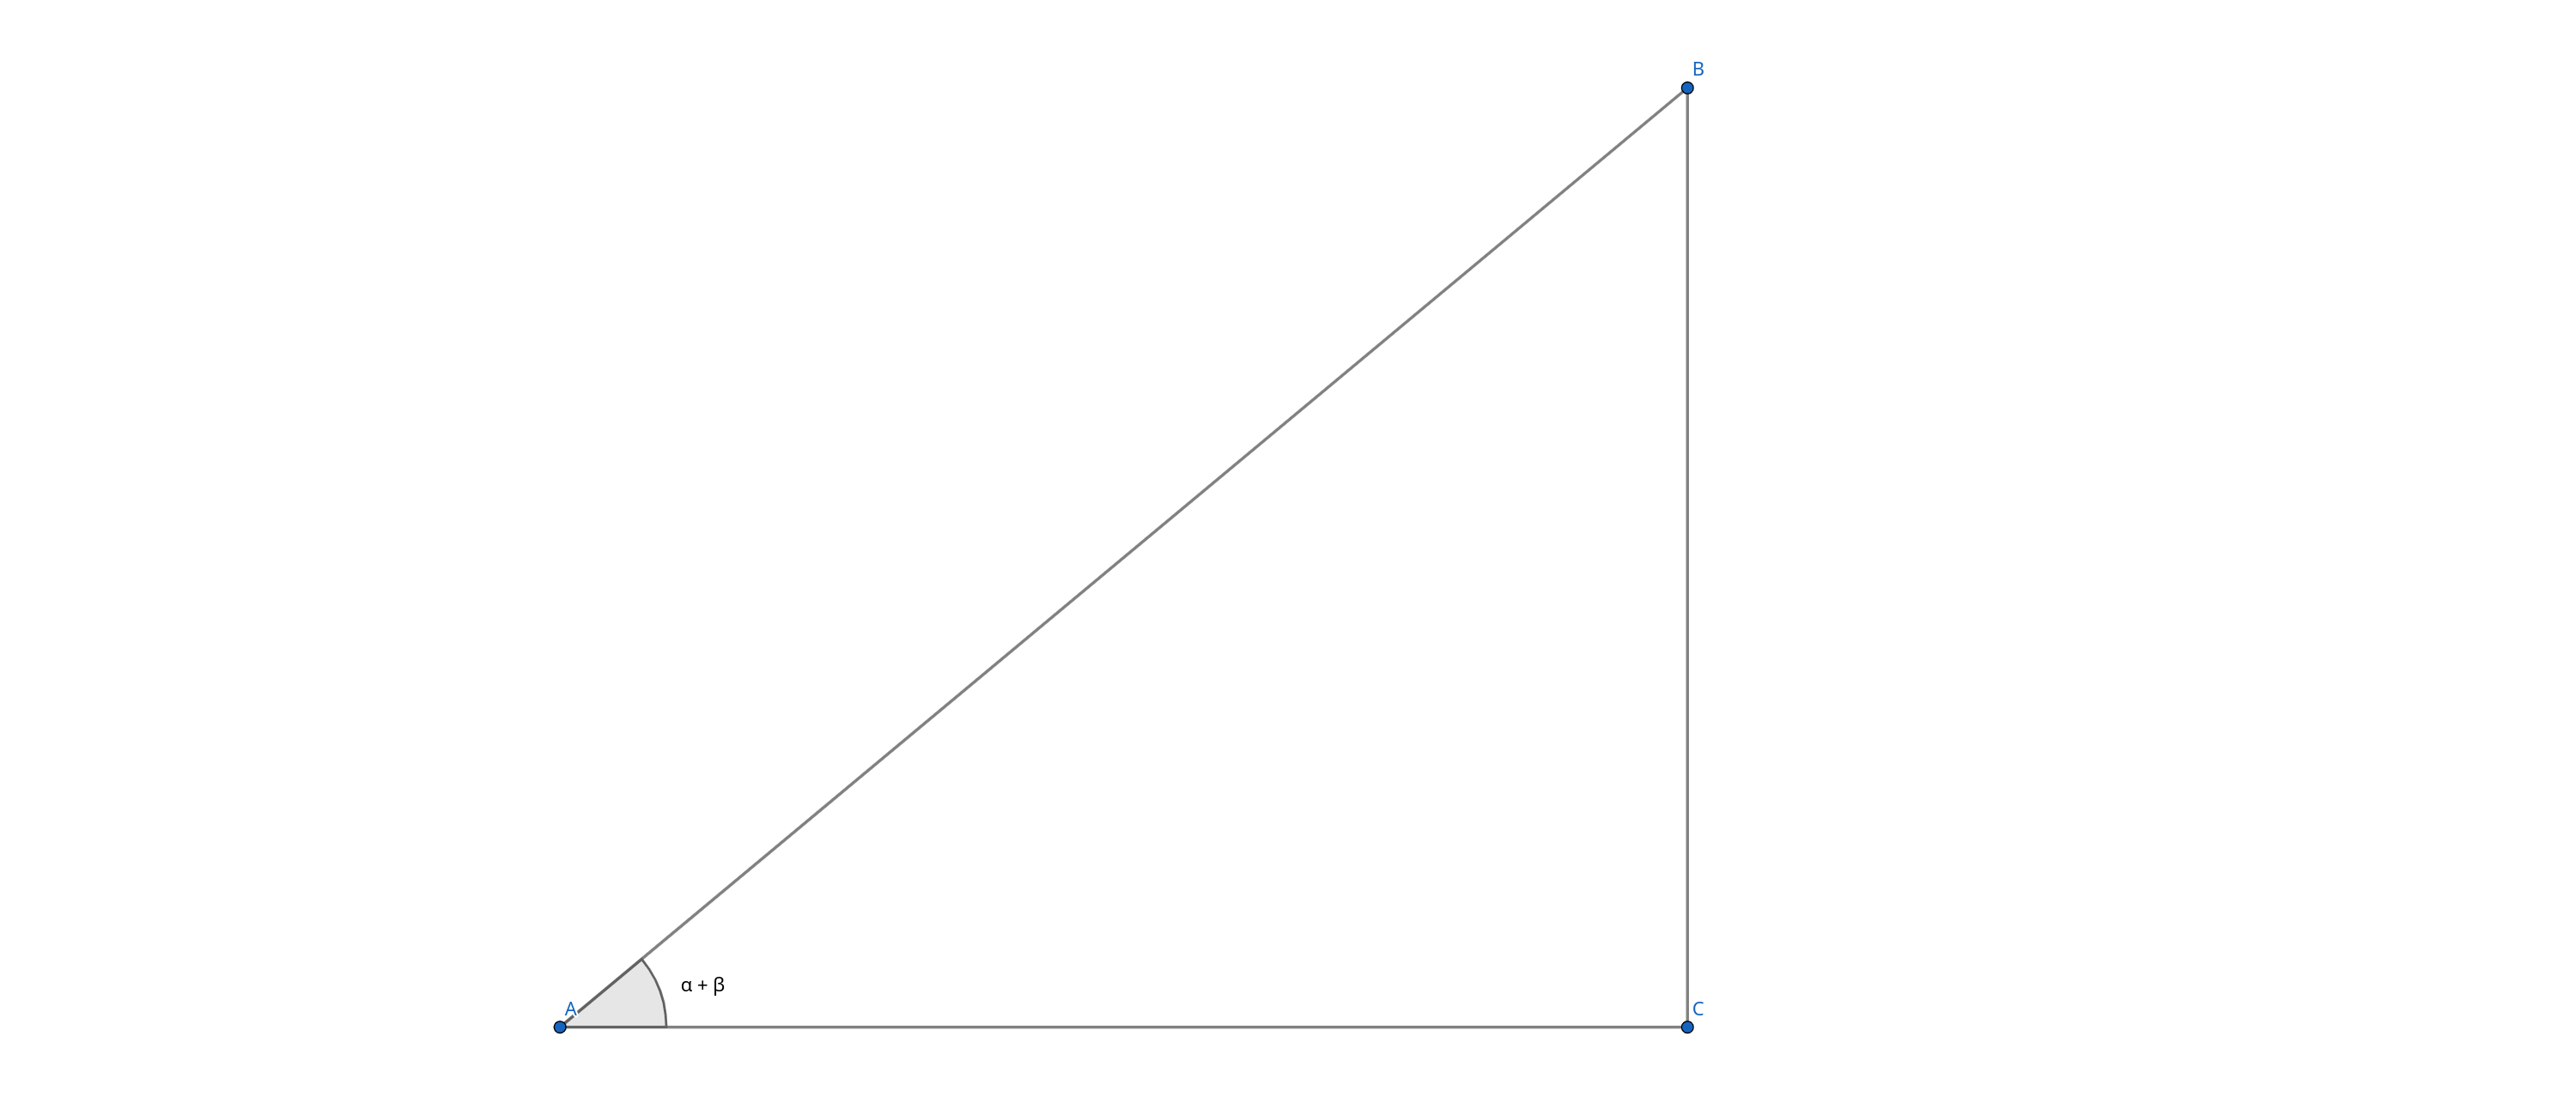
\includegraphics{trigo_sum_proof/initial.png}\\
Séparons l'angle $\sphericalangle A$ en deux ($\alpha$ et $\beta$).\\
Nous pouvons ainsi creer deux nouveaux triangles rectangles, ABF et AHF.\\
ACFG est composé de deux triangles semblables, donc $\sphericalangle ABF = \sphericalangle BAC = \alpha$.\\
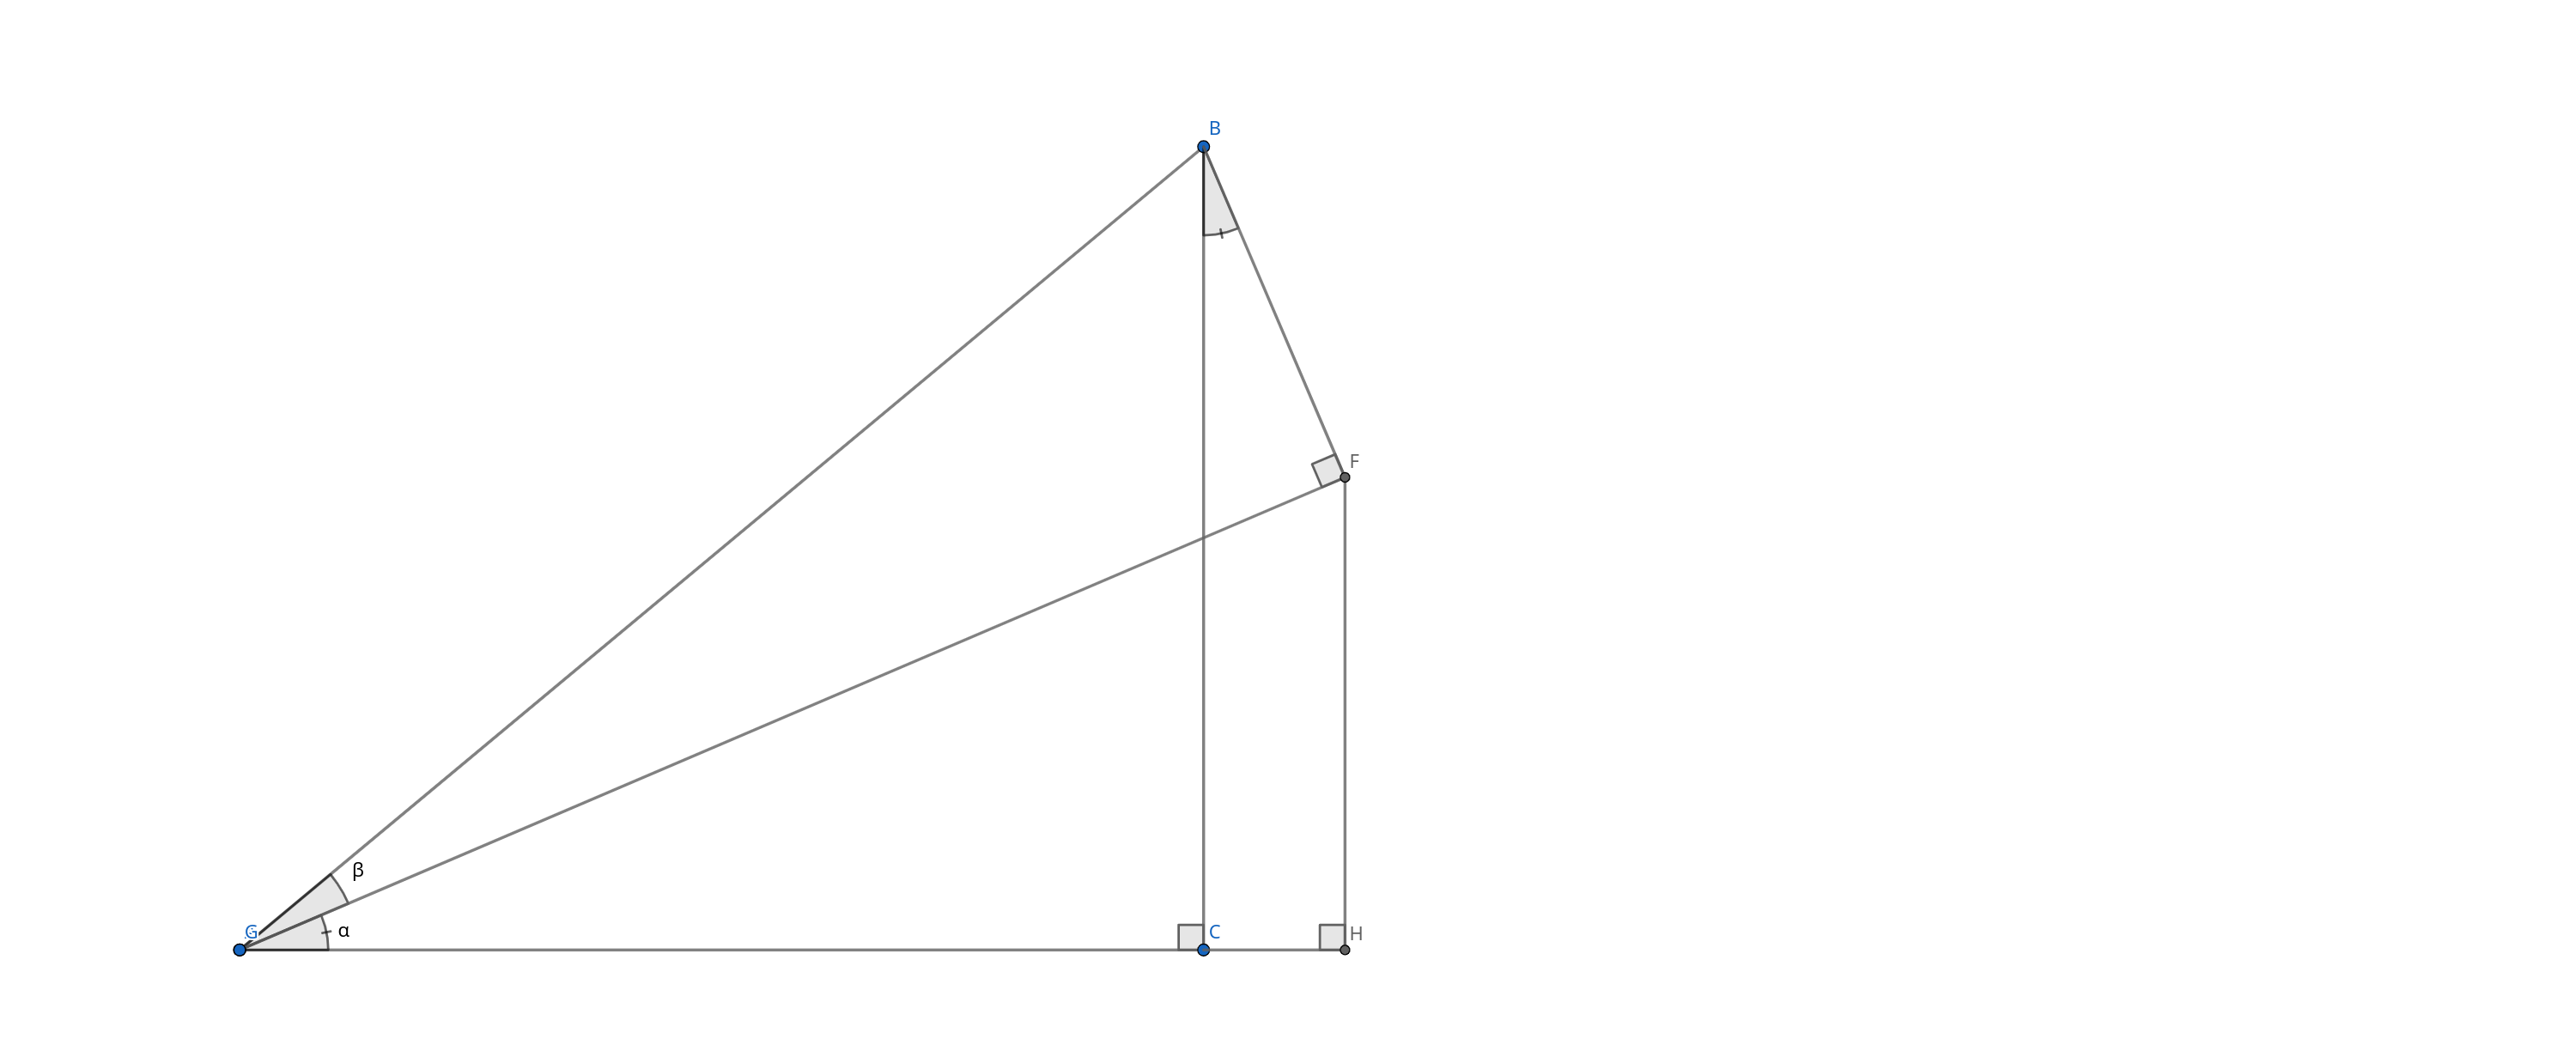
\includegraphics{trigo_sum_proof/mid.png}\\
Relions maintenant le point F a BC, créant un nouveau triangle rectangle BIF (comme du biff)\\
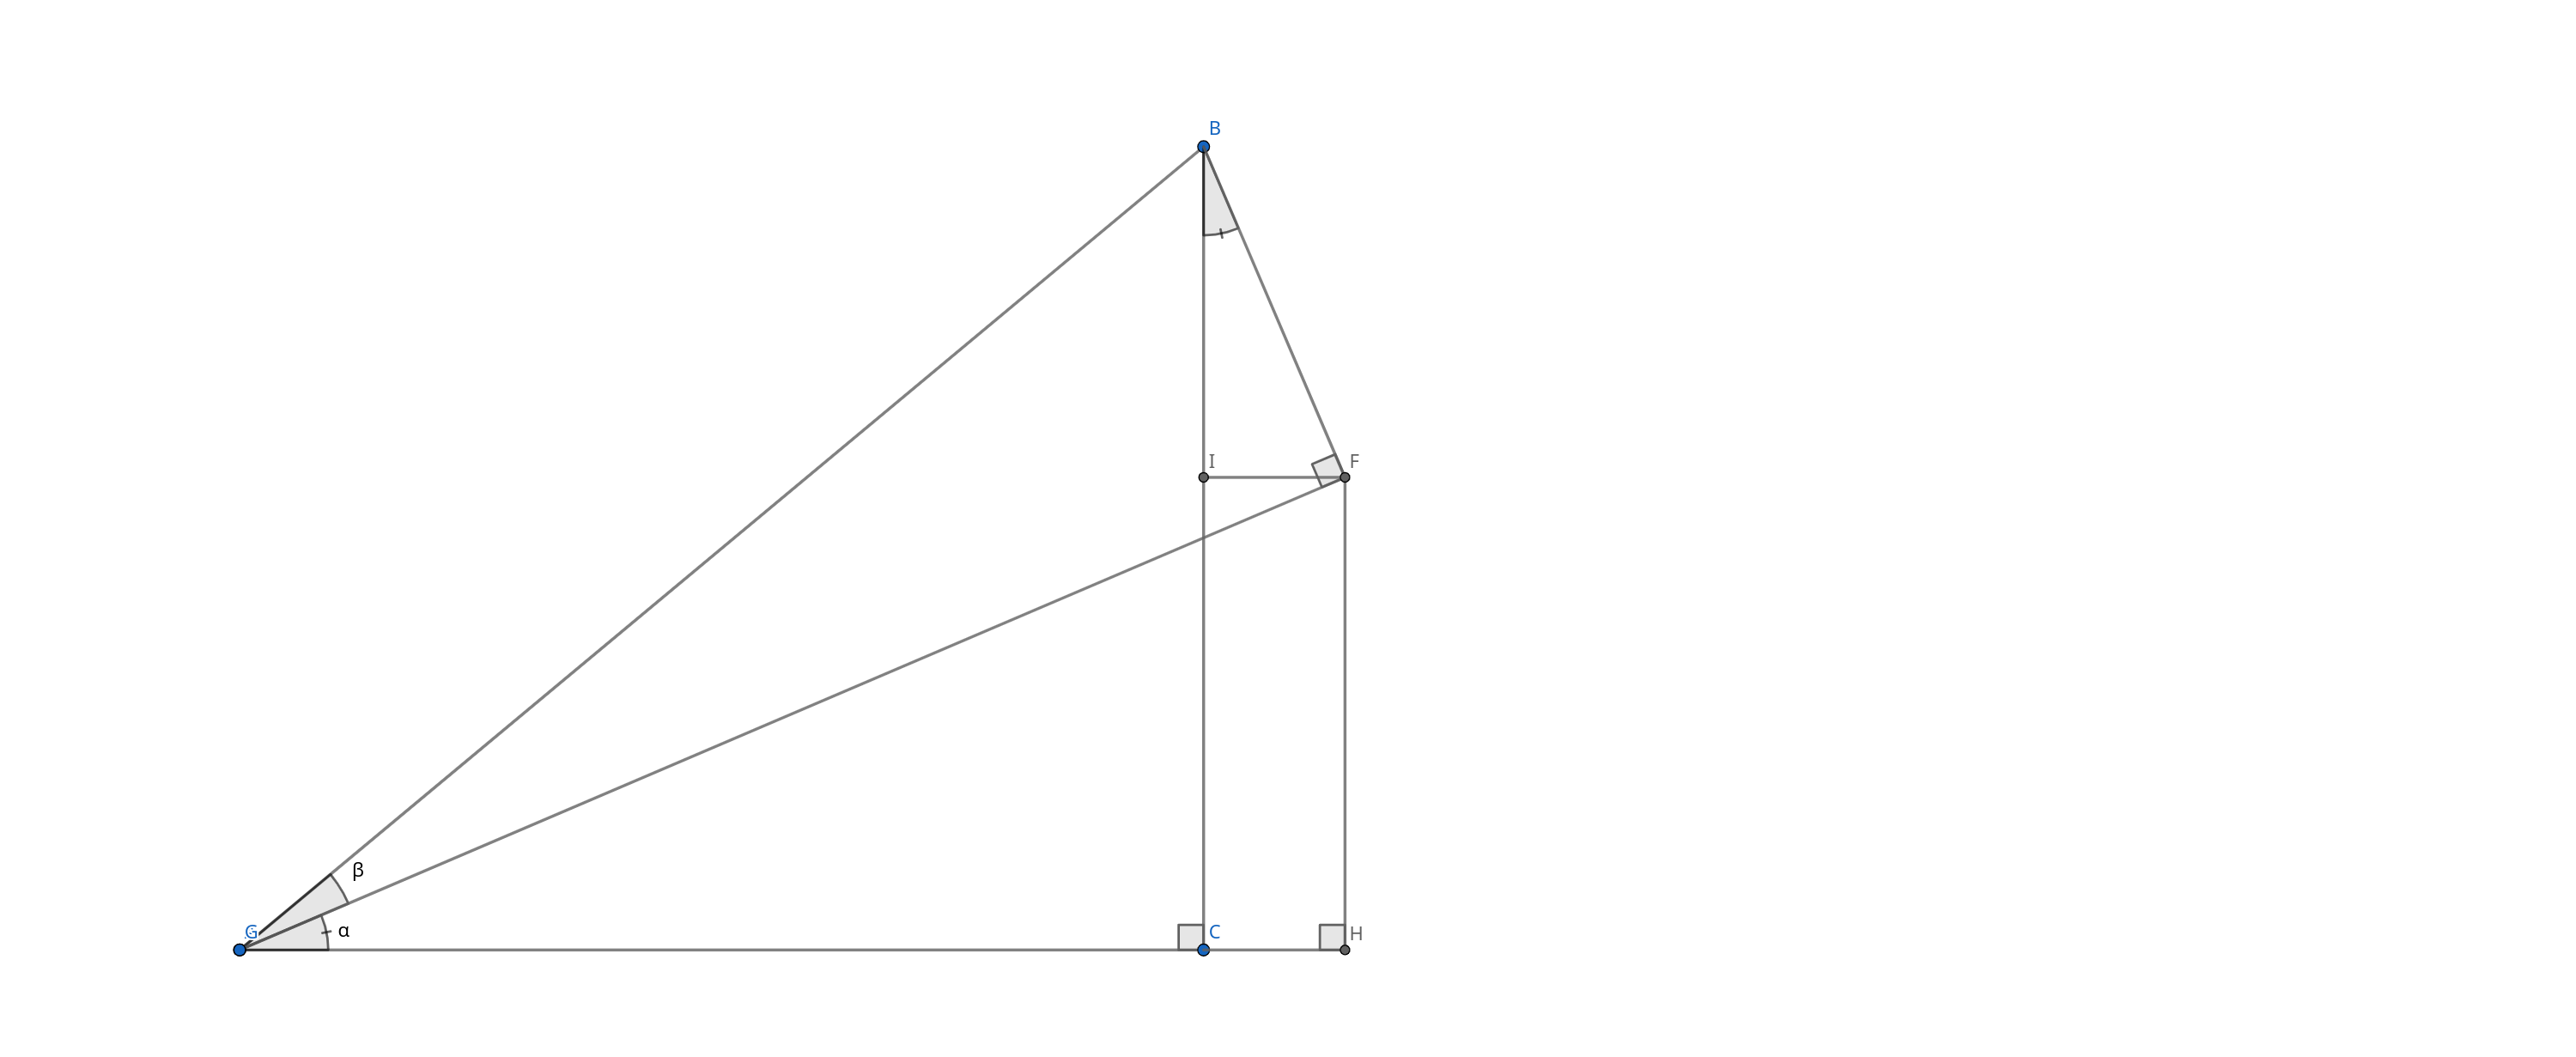
\includegraphics{trigo_sum_proof/last.png}\\
\\
Puisque $\text{AB} = 1$: \\
\begin{equation}
  \text{BF} = \sin\beta \\
\end{equation}
\begin{equation}
  \text{AF} = \cos\beta\\
\end{equation}
\begin{equation}
  \cos(\alpha+beta) = \text{AC}
\end{equation}
\begin{equation}
  \sin(\alpha+beta) = \text{BC}
\end{equation}
\begin{equation}
  \text{AH} = \cos\alpha * AF \Rightarrow \text{AH} = \cos\alpha * \cos\beta
\end{equation}
\begin{equation}
  \text{IF} = \sin\alpha * \text{BF} \Rightarrow \sin\alpha*\sin\beta
\end{equation}

\clearpage
Prouvons que $\sin(\alpha + \beta) = \sin\alpha\cos\beta + \cos\alpha\sin\beta$
\begin{align*}
  \sin(\alpha + \beta) &= \text{BC} \\
  \sin(\alpha + \beta) &= \text{BI} + \text{FH} \\
  \intertext{or}
  \cos\alpha = \frac{\text{BI}}{\text{BF}} &\Rightarrow \text{BI} = \cos\alpha * \text{BF}\\
  \sin\alpha = \frac{\text{FH}}{\text{AF}} & \Rightarrow \text{FH} = \sin\alpha * \text{AF}\\
  \intertext{et}
  \text{BF} &= \sin\beta \\
  \text{AF} &= \cos\beta\\
  \intertext{donc}
  \text{BI} &= \cos\alpha * \sin\beta\\
  \text{FH} &= \sin\alpha * \cos\beta\\
  \intertext{Ainsi}
  \sin(\alpha + \beta) &= \sin\alpha\cos\beta + \cos\alpha\sin\beta
\end{align*} 
De la même manière:\\
\begin{align*}
  \cos(\alpha+\beta) &= \text{AC}\\
  \cos(\alpha+\beta) &= \text{AH} - \text{IF}\\
  \cos(\alpha+\beta) &= \cos\alpha\cos\beta - \sin\alpha\sin\beta
\end{align*}
\\ 
Les soustractions reviennent juste a inverser le signe du milieu:\\
\begin{align*}
  \sin(\alpha-\beta) &= \sin\alpha\cos\beta - \cos\alpha\sin\beta\\
  \cos(\alpha-\beta) &= \cos\alpha\cos\beta + \sin\alpha\sin\beta
\end{align*}

\section{Angles $>$ 90\textdegree}
Les fonctions $\cos$ et $\sin$ ne se définissent que pour $0 < \alpha < 90$ \\
Pour calculer ces fonctions sur des angles en dehors de ces limites, il faut d'abord les ramener dans ces limites. \\
Puisque $\cos$ et $\sin$ sont des fonctions de cercle, il existe une symétrie.  \\

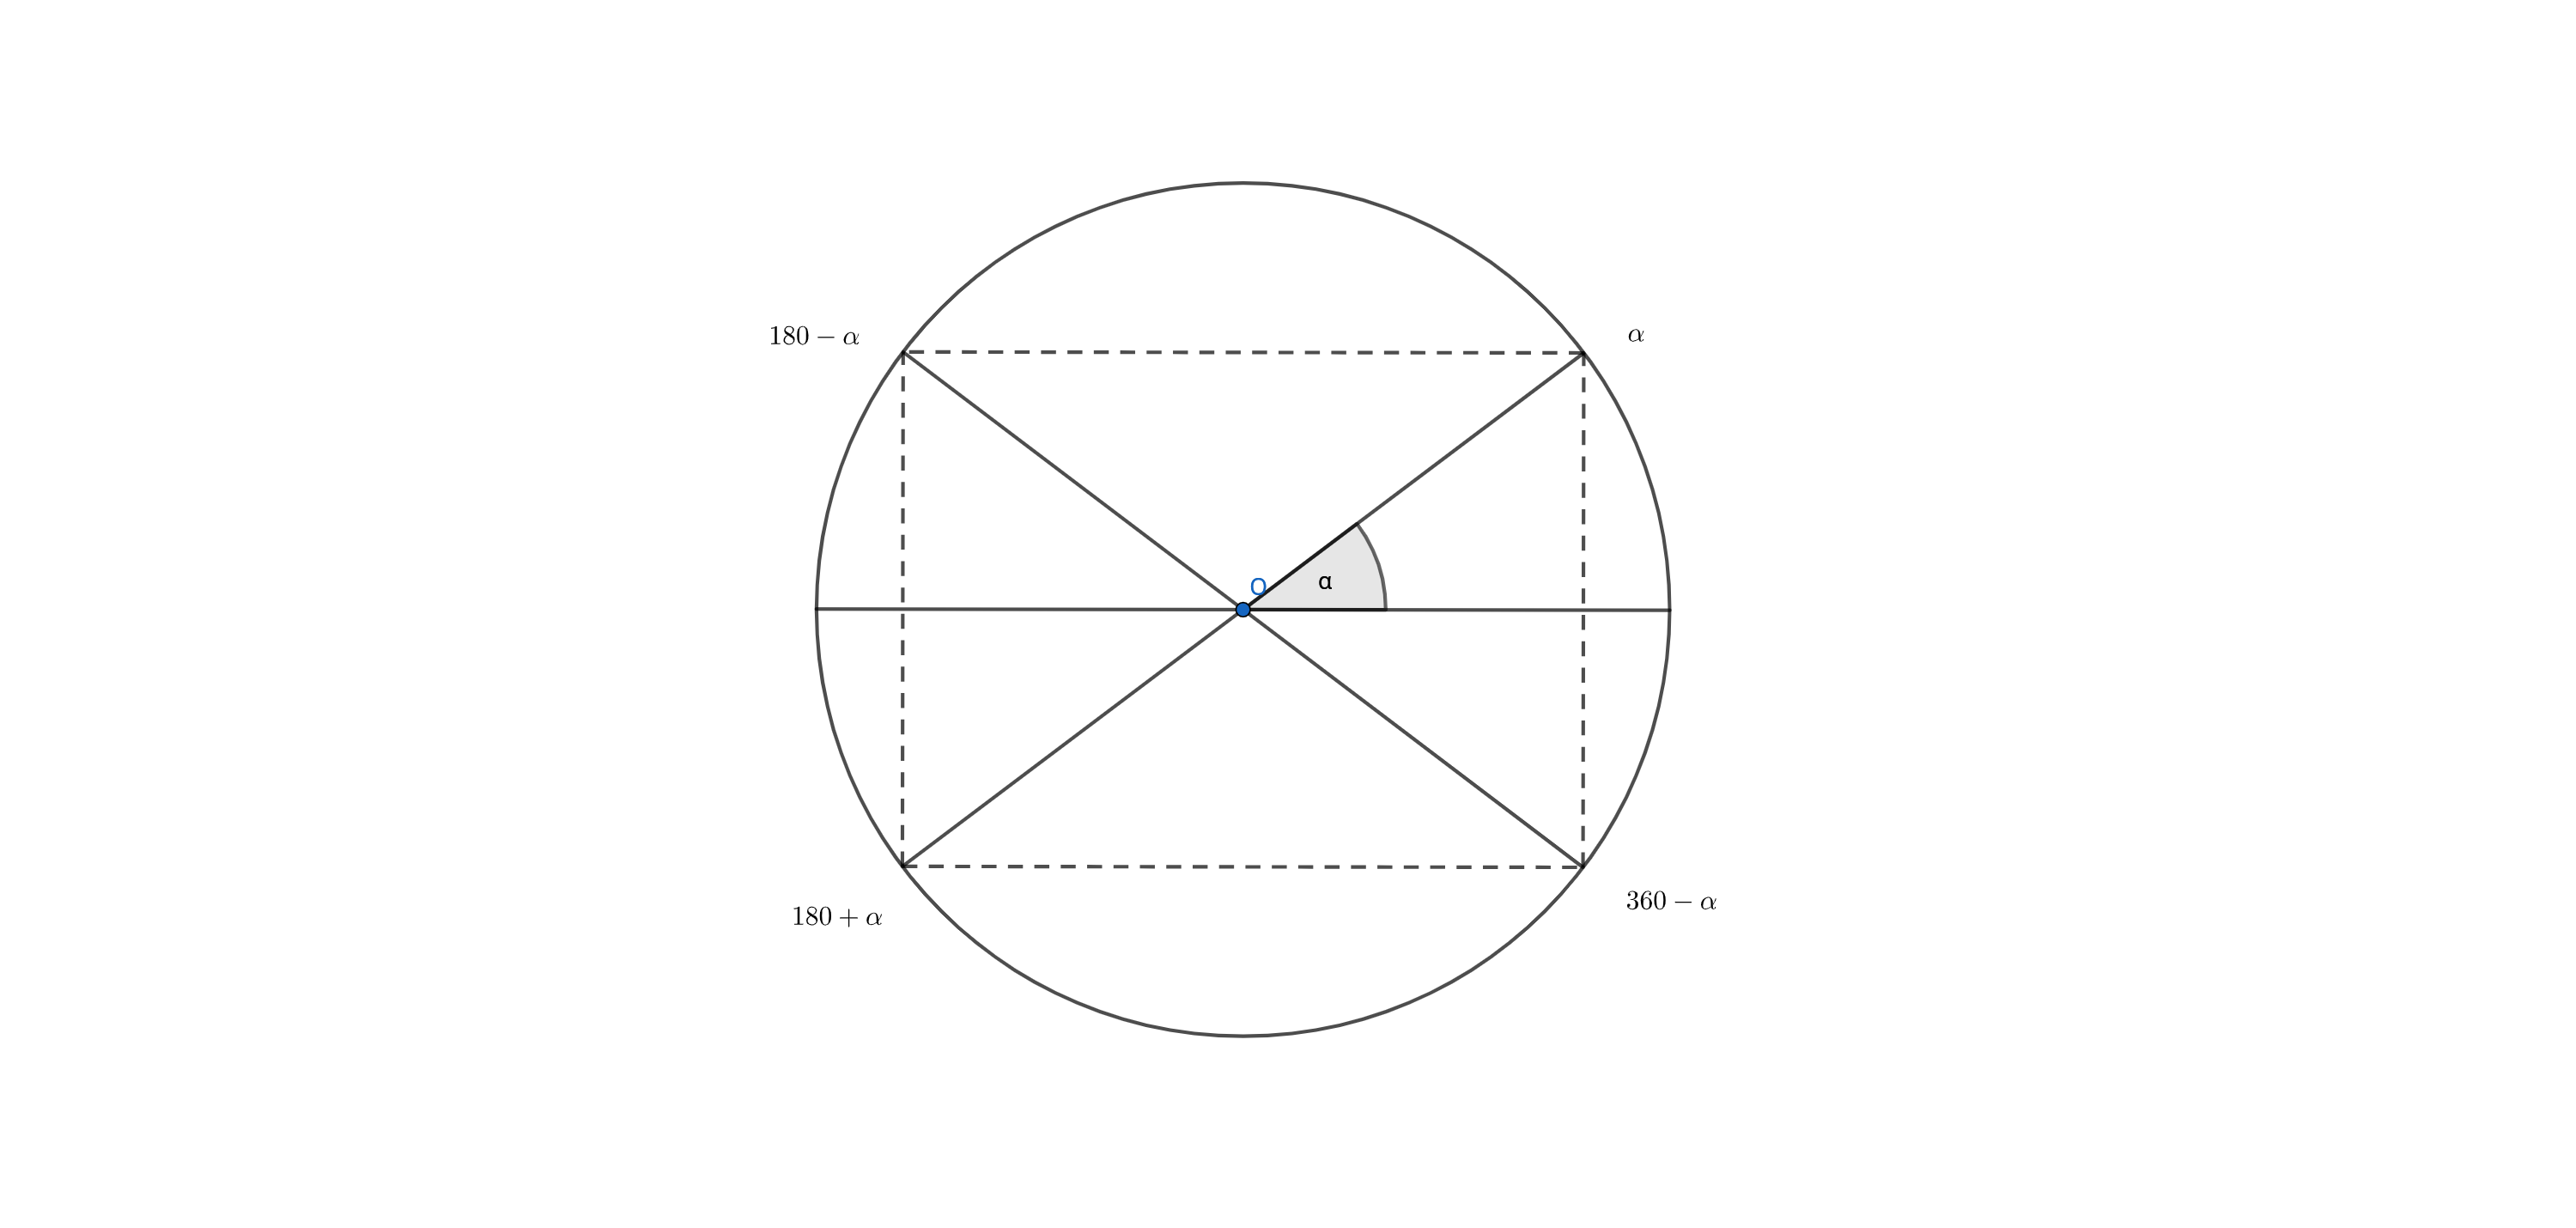
\includegraphics{circle_trigo_symetry.png}\\
Ainsi par exemple pour tout angle $\alpha$: $\cos(180-\alpha) = - \cos\alpha$.\\
Les seuls cas ou la valeur n'est pas transformée en négatif sont:\\
\begin{itemize}
  \item $\cos(360 - \alpha)$
  \item $\sin(180 - \alpha)$
  \item $\tan(180 + \alpha) $
  \item $\cot(180 + \alpha)$
\end{itemize}

\section{Radians}
Dans un cercle, on mesure un angle en radians selon la longueur de l'arc qu'il forme. Sa valeur en radians est égale a la longueur de l'arc divisée par le rayon $\frac{l}{R}$ tandis que sa valeur en degrés est définie par la longueur de l'arc divisée par 360 $\frac{l}{360}$.\\
Ainsi pour passer d'un angle de $\alpha$ degrés a sa valeur $x$ en radians, ou l'inverse, il existe l'équation suivante: \\
\begin{equation}
  \frac{x}{2\pi} = \frac{\alpha}{360}
\end{equation}

\subsection{Fonctions trigonométriques en radians}
Les relations entre les fonctions restent évidemment les mêmes.\\
\\
Pour chaque angle $x$, il existe un angle symétrique $\frac{\pi}{2} - x$ a l'intérieur du cadran qui inverse le $\sin$ et le $\cos$.\\
\begin{equation*}
  \sin(x) = \cos(\frac{\pi}{2} - x)
\end{equation*}
\begin{equation*}
  \cos(x) = \sin(\frac{\pi}{2} - x)
\end{equation*}
Idem pour $\tan$ et $\cot$.
\\
\textbf{Remarque perso:} Ajouter $\frac{\pi}{2}$ a $x$ revient a tourner le cercle de 90\textdegree vers la gauche.\\
\\
Puisque c'est un cercle, ajouter $2\pi$ a $x$ revient au même point, et ajouter $\pi$ a $x$ le fait passer a son opposé dans le cercle, donc:\\
\begin{align*}
  \sin(2\pi k + x) &= \sin(x)\\
  \cos(2\pi k + x) &= \cos(x)\\
  \\
  \tan(\pi k + x) &= \tan(x)\\
  \cot(\pi k + x) &= \cot(x)\\
\end{align*}


\subsection{Conversions courantes}
\begin{center}
  \renewcommand\arraystretch{1.5}
  \begin{tabular}{c | c | c | c | c | c }
    $\alpha$ & 0\textdegree & 30\textdegree & 45 \textdegree & 60 \textdegree  & 90 \textdegree\\
  \hline
    x & 0 & $\frac{\pi}{6}$ & $\frac{\pi}{4}$ & $\frac{\pi}{3}$ & $\frac{\pi}{2}$
\end{tabular}
\end{center}
  
\subsection{Symétrie}
1) $\pi + x$: Symétrie diagonale\\
2) $\pi - x$: Symétrie verticale\\
3) $2\pi - x$: Symétrie horizontale\\

\section{Autres formules}
\subsection{Avec un angle}
\begin{align*}
  \sin 2x &= 2\sin x\cos x\\
  \cos 2x &= \cos^2 x - \sin^2 x
\end{align*}
\begin{align*}
  1 + \cos 2x = 2 \cos^2 x
  1 - \cos 2x = 2 \sin^2 x
\end{align*}

\subsection{Avec deux angles}
Additions:\\
Pour les sinus: $2*\sin*\cos$, les signes de la fraction s'inversent si c'est un -
\begin{align*}
  \sin x + \sin y &= 2 *\sin(\frac{x+y}{2}) * \cos(\frac{x-y}{2})\\
  \sin x - \sin y &= 2 *\sin(\frac{x-y}{2}) * \cos(\frac{x+y}{2})\\
\end{align*}
Pour les cos: $2*\cos*\cos$ si +, $2*\sin*\sin$ si -, les signes ne s'inversent pas
\begin{align*}
  \cos x + \cos y &= 2 *\cos(\frac{x+y}{2}) * \cos(\frac{x-y}{2})\\
  \cos x - \cos y &= 2 *\sin(\frac{x+y}{2}) * \sin(\frac{x-y}{2})\\
\end{align*}
\\
Multiplications:\\
$\sin x*\cos y = \frac{1}{2}[\sin(x+y) + \sin(x - y)]$
$\sin x*\sin y = \frac{1}{2}[\cos(x+y) - \cos(x - y)]$
$\cos x*\cos y= \frac{1}{2}[\cos(x+y) + \cos(x - y)]$
  
  
\end{document}

